
% submission details
\newcommand{\deadlineTwoTime}{noon}
\newcommand{\deadlineTwoDate}{13 March 2020}
\newcommand{\submissionTwoURL}{https://tabula.warwick.ac.uk/coursework/submission/0a00dc0e-23b7-437a-9c6b-62ad4380bad1}


%\renewcommand{\instructions}{Due at \emph{\deadlineTime} on \emph{\deadlineDate}.}

\cleardoublepage
\chapter{Coursework II}

\section{Scratch clone}

Scratch\footnote{\url{https://scratch.mit.edu/}} is a visual programming language designed to teach programming to children in a fun and graphical way. Programs in Scratch are built by arranging blocks that correspond to different syntactic constructs and connecting them like puzzle pieces. The tool is free to use so you can give it a go if you want! To give you an idea of what it looks like, here is a screenshot of Pac-Man built in Scratch running on a Raspberry Pi:

\begin{center}
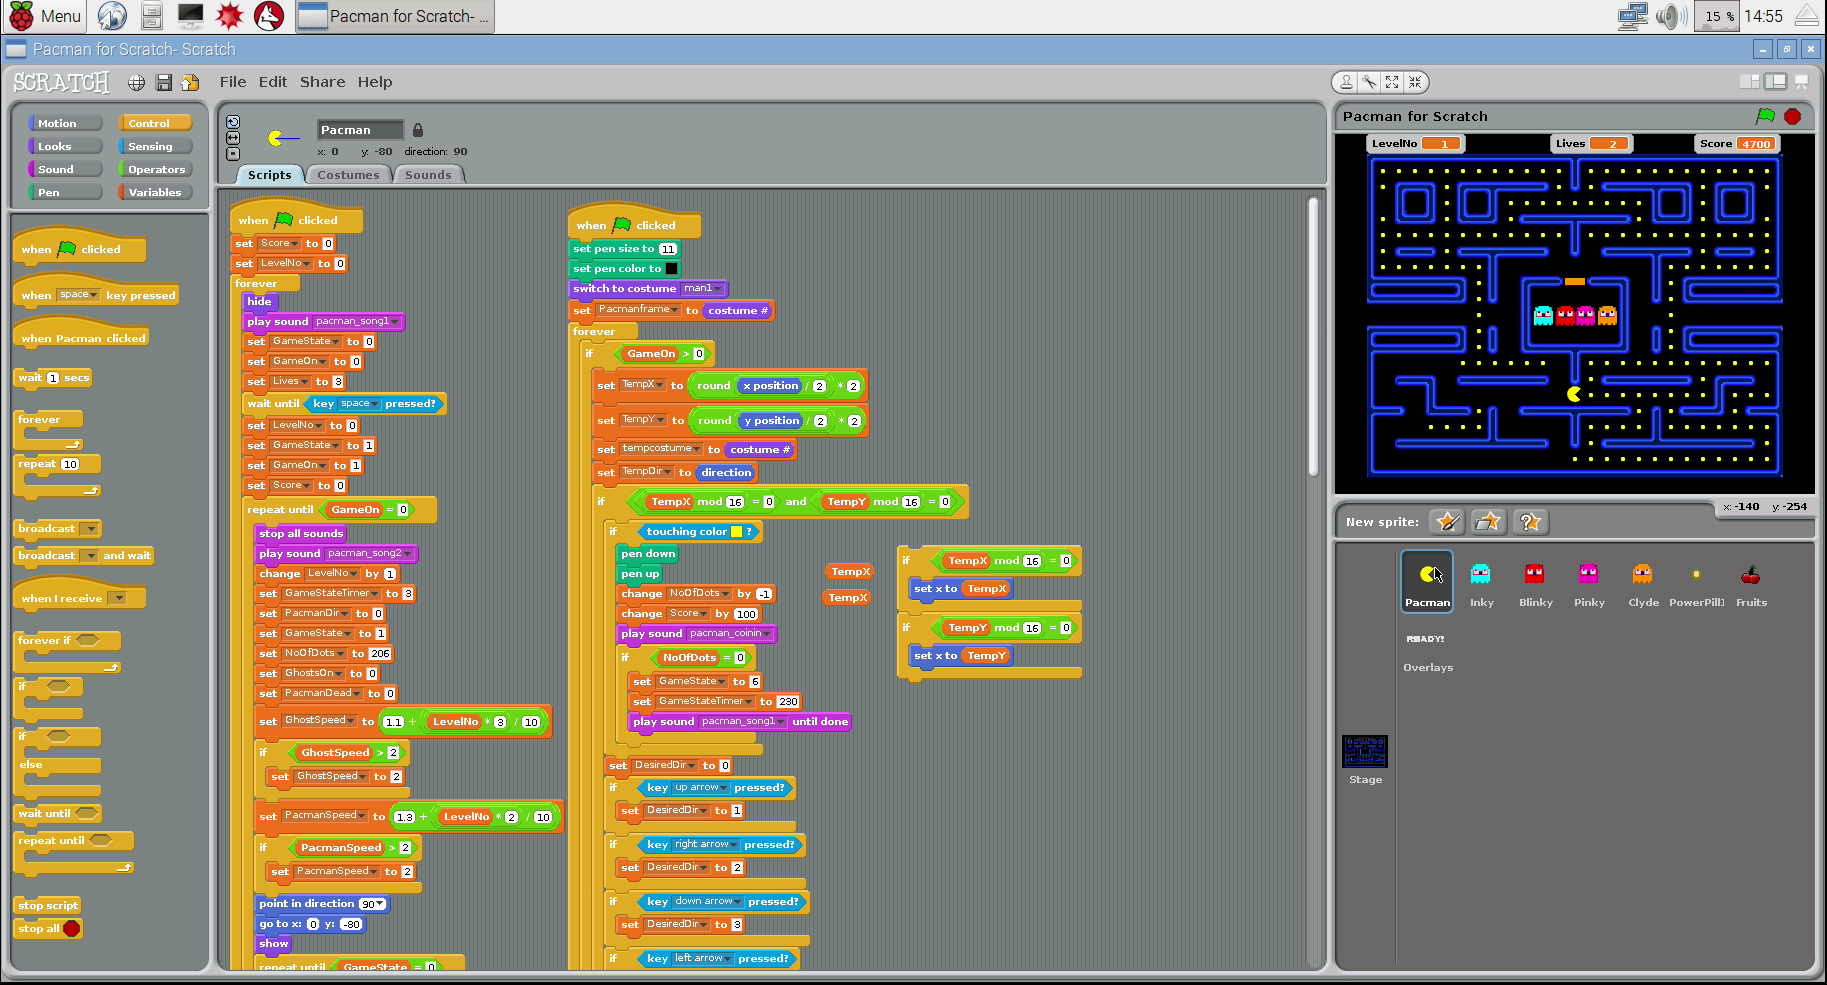
\includegraphics[width=390px]{cswk/scratch_rpi.png}
\end{center}

The goal of this coursework is to implement a simple clone of Scratch. Our clone will consist of two components:
\begin{enumerate}
    \item A web-based interface which allows users to construct simple programs visually. This is written in JavaScript and is already implemented for you.
    \item A Haskell program which handles the evaluation of such programs. This is partially implemented and you will have to finish it.
\end{enumerate}
Your task is to complete the part of the Haskell program responsible for evaluating programs -- in other words, you have to write an \emph{interpreter}.

An interpreter is a program which, given some representation of a program as argument, evaluates it. To illustrate this idea, a Haskell implementation of an interpreter for a simple expression language is shown below:
\begin{minted}{haskell}
data Expr = Val Int | Add Expr Expr 

eval :: Expr -> Int
eval (Val n)   = n
eval (Add l r) = eval l + eval r
\end{minted}
Expressions in the language represented by \haskellIn{Expr} consist of the addition operator and integer values. The \haskellIn{eval} function is the interpreter for this language, which determines the value of a given expression.

\section{Getting started}

In order to get started with the coursework, you need to get hold of the skeleton code and ensure that it compiles successfully. 

\subsection{Obtaining the skeleton code}

There are three different ways in which you can obtain the skeleton code for this coursework, which are all explained below alongside their advantages and disadvantages:

\paragraph{Option A: Private fork} By following the GitHub Classroom link below, you can create a private fork of our git repository with the skeleton code. This requires a GitHub account, but has the advantage that you have your own private copy of our repository on GitHub that you can write to. That would allow then you to work easily share your work between machines in the labs and at home:
\begin{center}
	\url{https://classroom.github.com/a/4aP_BvWI}
\end{center}
Once you have accepted the assignment, you can then clone your fork of the skeleton code to your machine with the usual \bashIn{git clone} command where \texttt{\small [username]} is your GitHub username:
\begin{minted}{bash}
$ git clone https://github.com/fpclass/1920-cswk2-[username]
\end{minted}

\paragraph{Option B: Clone} If you do not wish to create a GitHub account or host a copy of your repository there, then you could instead just clone our repository with:
\begin{minted}{bash}
$ git clone https://github.com/fpclass/scratch-clone
\end{minted}
You will be able to \bashIn{git commit} changes to your local copy of the repository, but you will not be able to \bashIn{git push} them. This is sufficient if you are only planning to work on the coursework from one place (\emph{e.g.} only the lab machines but not your personal computer).

\paragraph{Option C: Archive} If GitHub should be unavailable or you do not have \bashIn{git} installed your machine, you can download a \texttt{\small .zip} file with the skeleton code from the module website.

\subsection{Working with the skeleton code}

The code should compile out of the box. You can test this by running:
\begin{minted}{bash}
$ stack build
\end{minted}
To start the program, you should run the following:
\begin{minted}{text}
$ stack exec scratch-clone
Starting web server...
Started. Press any key to quit.
\end{minted}
In order to view the user interface, open your web browser and navigate to\footnote{If, for whatever reason, port 8000 is unavailable on your machine, you can change this by modifying the definition of \haskellIn{main} in \texttt{\small src/Main.hs}.}:
\begin{center}
\url{http://localhost:8000/}
\end{center}
You can drag together programs using building blocks from the toolbox on the left. However, if you click ``Evaluate'' at the top right corner of the screen, you will get an error since the interpreter is not yet implemented.

The skeleton code contains a bunch of files, most of which you do not need to touch initially. The most important file is \texttt{\small src/Interpreter.hs} which contains the definitions you will need to complete to get the interpreter to work. There are some definitions to get you started. A program's initial memory is represented as a list of pairs. Each pair represents one variable, consisting of a name of type \haskellIn{String} and a value of type \haskellIn{Int}:
\begin{minted}{haskell}
type Memory = [(String, Int)]
\end{minted}
It is possible for things to go wrong when interpreting a program. There are two sorts of errors which may occur. These are represented by the following data type:
\begin{minted}{haskell}
data Err = DivByZeroError | UninitialisedMemory String
\end{minted}
The types representing the language itself are defined in \texttt{\small src/Language.hs}. You should have a look at this file yourself, but an overview of the most important types is below. A program is a list of statements:
\begin{minted}{haskell}
type Program = [Stmt]
\end{minted}
There are three different forms of statements: 
\begin{minted}{haskell}
data Stmt = AssignStmt String Expr
          | IfStmt Expr [Stmt] [(Expr,[Stmt])] [Stmt]
          | RepeatStmt Expr [Stmt]
\end{minted}
Assignments, represented by the \haskellIn{AssignStmt} constructor, consists of the name of the variable that we are assigning a value to and the expression whose value we should assign to the variable. 

If statements, represented by the \haskellIn{IfStmt}, are more complicated. The first expression is the condition of the ``if'' clause. The list of statements which follows is the code that should be run if the condition is true. The list of pairs of expressions and lists of statements represent ``if else'' clauses. Finally, the last list of statements represents the ``else'' clause.

Repeat statements, represented by the \haskellIn{RepeatStmt} constructor, consist of an expression which determines how many times the repeat loop should be executed and a list of statements which represent the body of the repeat statement.

There are also three forms of expressions:
\begin{minted}{haskell}
data Expr = ValE Int
          | VarE String
          | BinOpE Op Expr Expr
\end{minted}
The \haskellIn{ValE} constructor represents integer values, the \haskellIn{VarE} constructor represents variables, and the \haskellIn{BinOpE} constructor generalises binary operators. The \haskellIn{Op} data type in \texttt{\small src/Language.hs} enumerates all available operators.

\section{Task}

Complete the definition of the \haskellIn{interpret} function in \texttt{\small src/Interpreter.hs} so that all values of type \haskellIn{Program} can be evaluated correctly according to the rules described below. Programs are sequences of statements and should be evaluated in the order in which they are given. We illustrate all rules for the language with screenshots of the GUI and the expected results:

\begin{center}
	\begin{longtable}[t]{|c|p{5cm}|}
		\hline 
		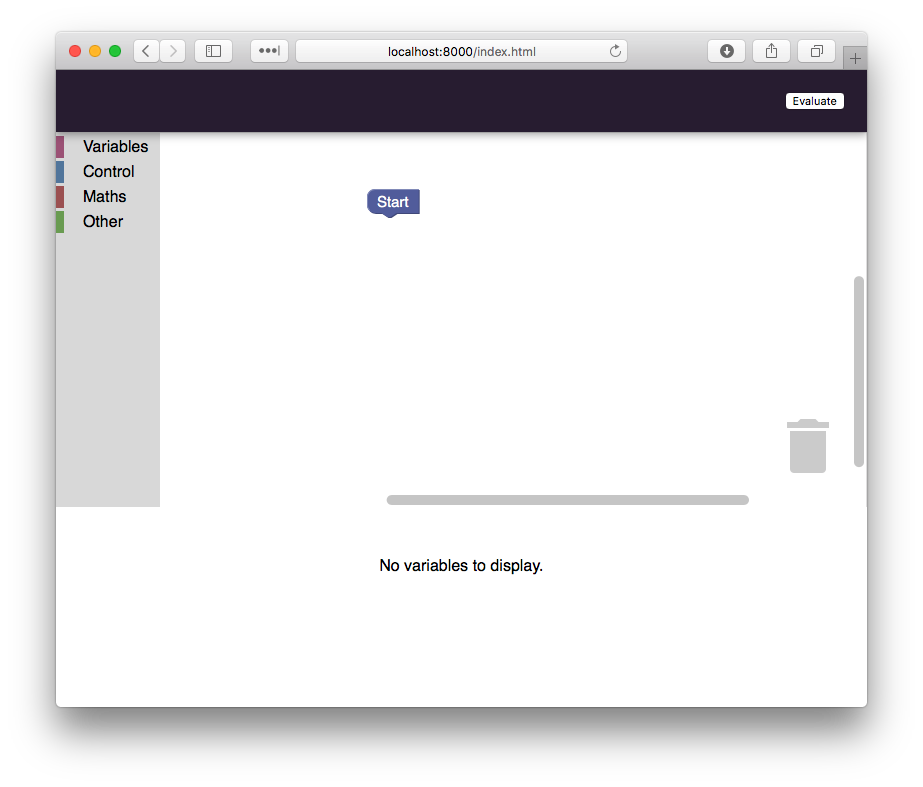
\includegraphics[align=t,width=250px]{cswk/0-empty.png} & 
		If the program is empty as shown in the screenshot, the initial contents of the memory should be returned. \\ \hline 
		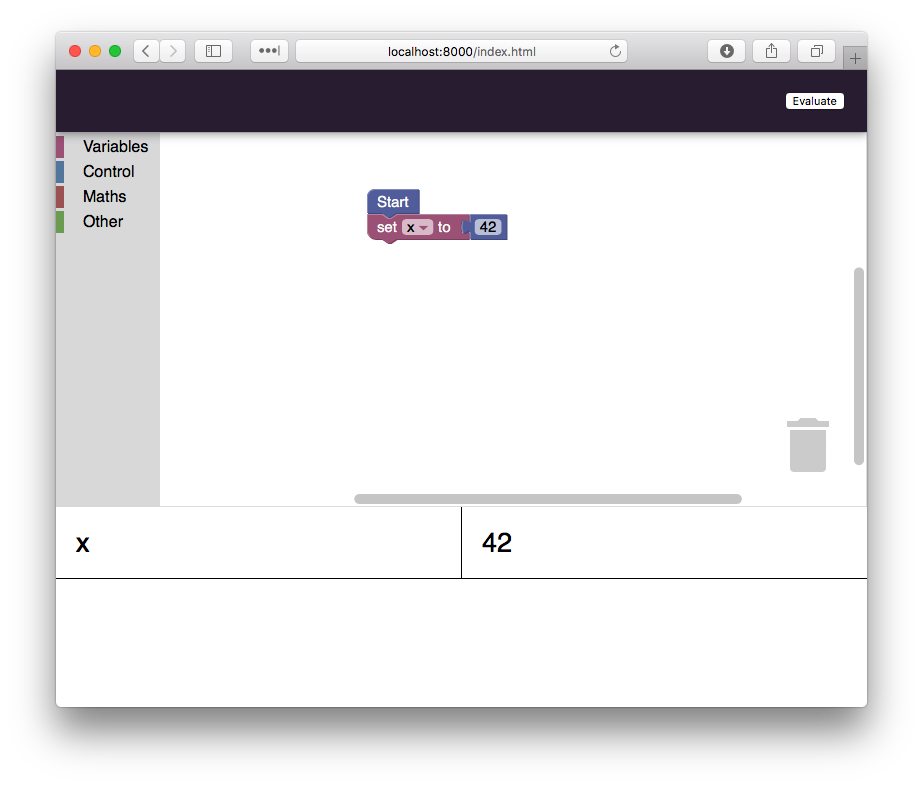
\includegraphics[align=t,width=250px]{cswk/1-assignment.png} & 
		Assignment statements should update the memory to the value of their expression. \\ \hline 
		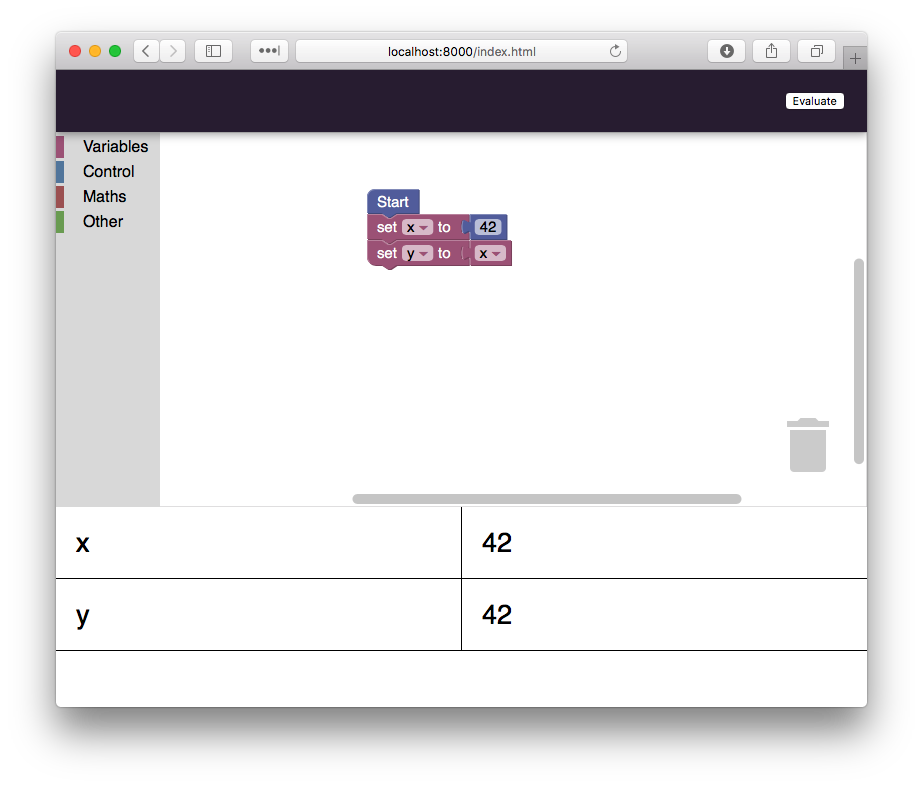
\includegraphics[align=t,width=250px]{cswk/2-loading.png} &
		If a variable occurs in an expression, the corresponding value should be loaded from memory. \\ \hline 
		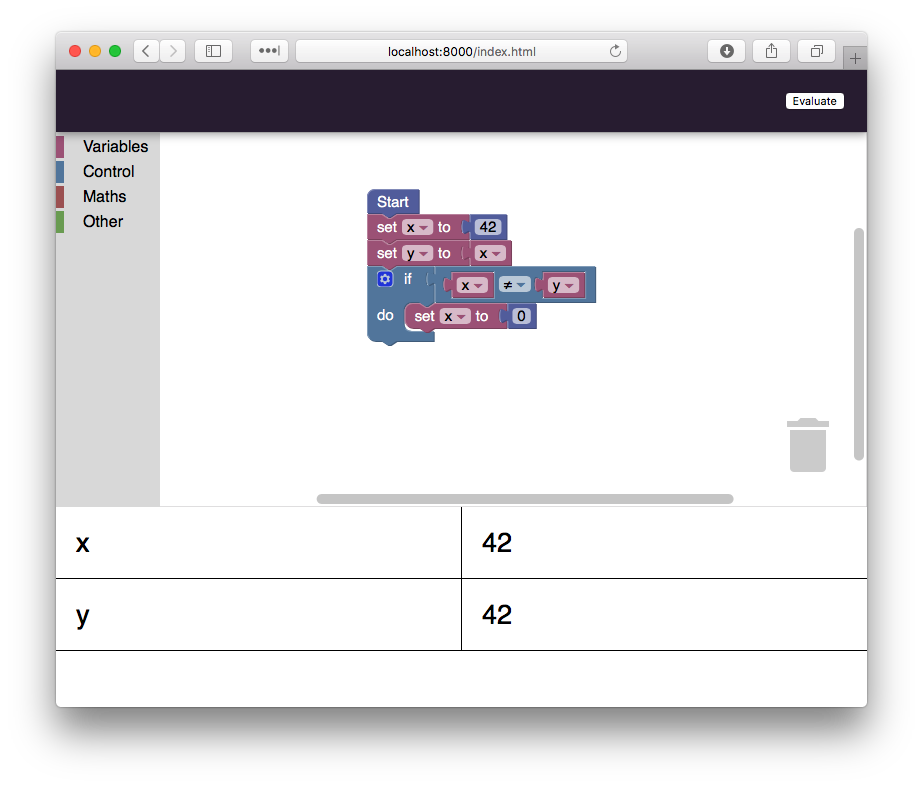
\includegraphics[align=t,width=250px]{cswk/3-if.png} &
		If the condition of an if statement is true (\emph{i.e.} any non-zero value), then the body of the if clause should be executed. \\ \hline
		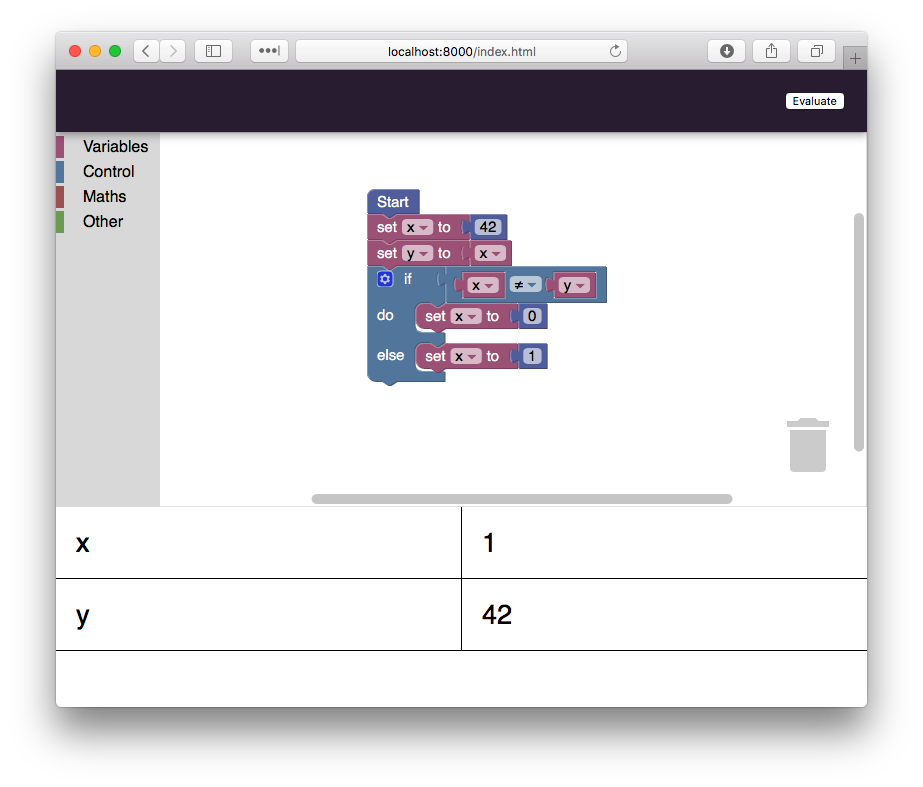
\includegraphics[align=t,width=250px]{cswk/4-else.png} &
		If the condition of an if statement is false (\emph{i.e.} it evaluates to zero), then the body of the else clause should be executed. \\ \hline 
		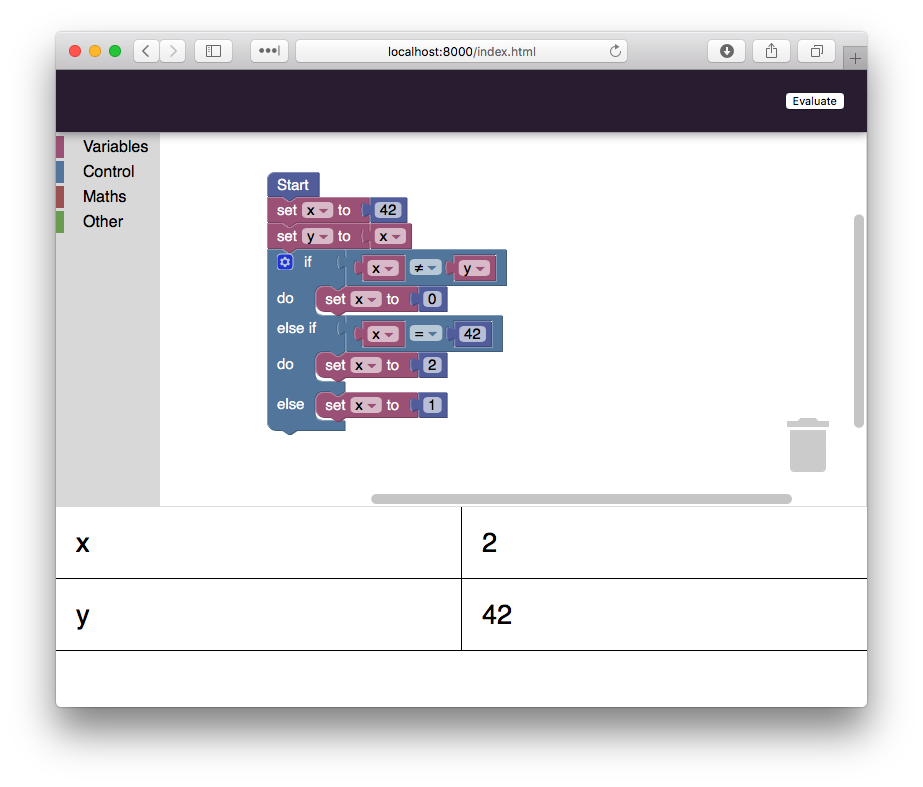
\includegraphics[align=t,width=250px]{cswk/5-ifelse.png} &
		If there are if else clauses present, their conditions should be checked in order after that of the main if clause. If one of them is true, then the corresponding body should be executed. \\ \hline
		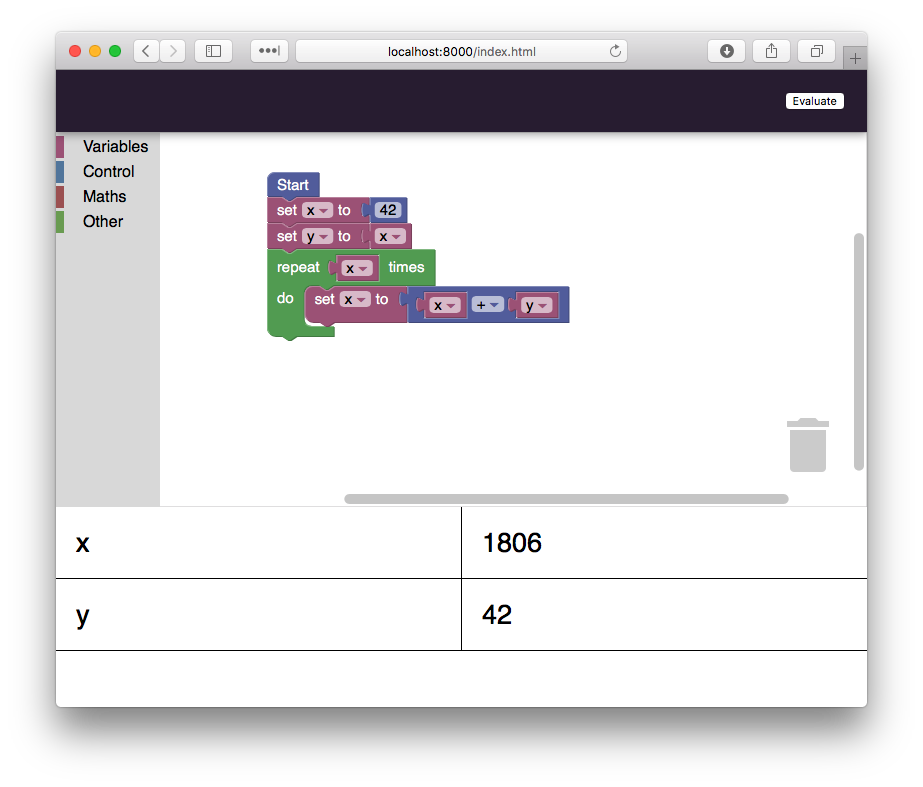
\includegraphics[align=t,width=250px]{cswk/6-repeat.png} &
		Repeat statements evaluate an expression to determine how many times they should run. The body of the repeat statement is then executed that many times. \\ \hline 
		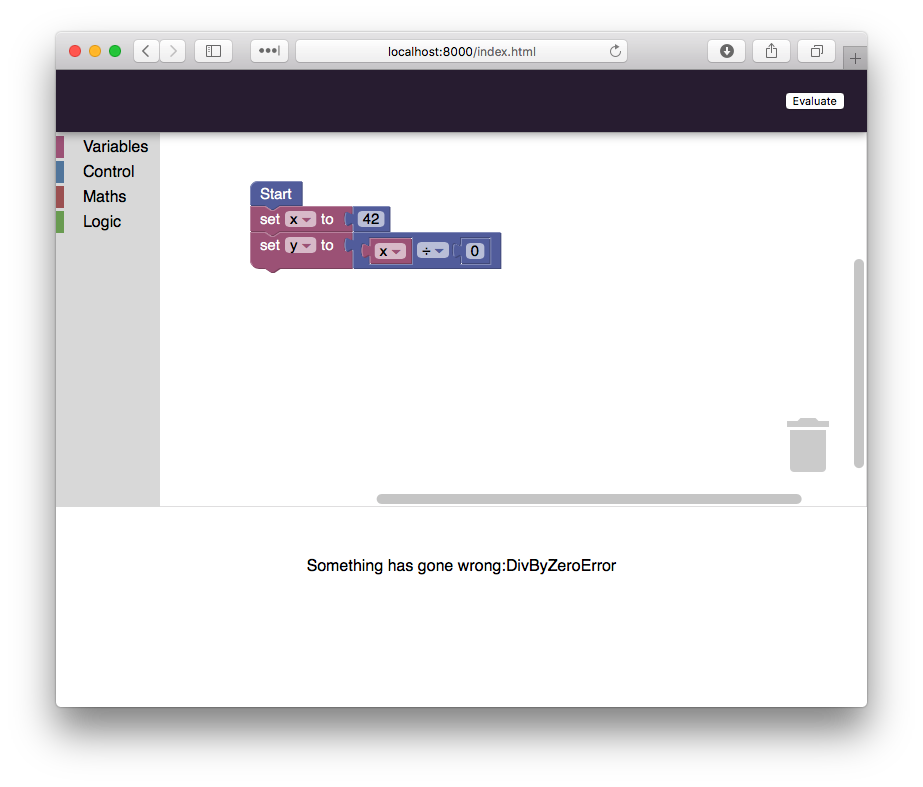
\includegraphics[align=t,width=250px]{cswk/7-divbyzero.png} &
		If a division by zero is attempted, the corresponding error should be returned. \emph{I.e.} \haskellIn{Left DivByZeroError} \\ \hline
	\end{longtable}
\end{center}
There are some details to look out for:
\begin{itemize}
	\item Internally, logic operators should evaluate to $0$ if false or a non-zero value if true. All numeric values other than $0$ should be treated as true.
	\item If an attempt is made to read from a variable which is not in the memory, then the corresponding error should be returned.
	\item Expressions can be nested arbitrarily deep and expressions of arbitrary complexity may appear in any place where expressions are expected.
	\item Errors can arise almost anywhere and should be propagated properly.
\end{itemize}

Running \texttt{\small stack test} will give you a rough indication of how complete your solution is. Running \bashIn{stack bench} will benchmark your code.

%-----------------------------------------------------------

\section{Originality \& academic practice}

This coursework is an individual assignment and the work you submit must be entirely your own work. Students are expected to be familiar with the departmental Student Handbook as well as applicable university regulations. The ``Cheating and Plagiarism'' section on the handbook page about coursework is particularly relevant:
\begin{center}\small
	\url{https://warwick.ac.uk/fac/sci/dcs/teaching/handbook/coursework/}
\end{center}
Examples of what is not acceptable in the context of this assignment include, but are not limited to, the following:
\begin{itemize}
	\item Collaborating with others, for example by sharing code, looking at other people's code, or discussing implementation details such as which functions you used to implement a particular definition. 
	
	\item Copying or adapting code from web sources such as Stack Overflow, GitHub, etc. without attribution. This includes taking code written in other programming languages and translating it to Haskell. You may do this if you include a correct attribution to the source in e.g. a comment in your file, but note that you can only be awarded marks for work you have done yourself. 
\end{itemize}

\section{Marking \& submission}

This coursework is worth 25\% of the overall module mark. It will be marked out of 100\% as follows:
\begin{itemize}
	\item 20\% for \emph{correctness}. You gain full marks here if all parts of the coursework have been attempted and are correct. You may use \bashIn{stack test} as a rough indication for whether this is the case, but there are some things the unit tests do not test for, so you should construct programs in the scratch clone and ensure that everything works as described.
	
	\item 20\% for \emph{documented understanding}. You should document your code with comments and explain how it works. You gain full marks if all code is documented and explained sufficiently well so that someone who is unfamiliar with your code can understand it.
	
	\item 20\% for \emph{elegance}. Definitions should be concise and readable, new functions should be introduced where needed, existing library functions used when applicable, monads used where possible, etc. 
	
	\item 20\% for \emph{performance and efficiency}. To do well here, you need to use sensible data structures and your functions should perform as little redundant computation as possible. In your comments, you must also discuss what you have done to test your solution's performance and what you have tried to improve it. You can test performance by running \bashIn{stack bench} on different versions of your code to see how they compare. 
	
	\item 20\% for \emph{improvements and extensions}. This is an opportunity for you to demonstrate creativity and advanced understanding. You could achieve this in many different ways, such as adding additional unit tests, functionality, improved algorithms, etc. You may wish to modify \texttt{\small exe/Main.hs} as well as other source files or even add new ones. You could also prove some properties about your interpreter on paper. The amount of marks awarded will depend on the complexity and creativity of your extension(s) and improvement(s).
\end{itemize}
Submit a \texttt{\small .zip} or \texttt{\small .tar.gz} archive of the whole, completed project (not just \texttt{\small Interpreter.hs}) through Tabula by \deadlineTwoTime\ on \deadlineTwoDate:

\begin{center} 
\url{\submissionTwoURL}
\end{center}